% !TEX program = xelatex
% 中证指数 · 中文金融刊物 A0 竖版海报（841mm × 1189mm）
\documentclass[UTF8,fontset=mac,11pt]{ctexart}
\usepackage{geometry}
\geometry{paperwidth=841mm,paperheight=1189mm,margin=0mm,footskip=0pt}

\usepackage{fontspec}
\setmainfont{Palatino}
\usepackage{unicode-math}
\setmathfont{texgyrepagella-math.otf}
\usepackage{amsmath}
\usepackage{xcolor}
\usepackage{tikz}
\usetikzlibrary{arrows.meta,positioning,calc,fit,backgrounds}
\usepackage{booktabs,array,tabularx,ragged2e,colortbl}
\usepackage{tcolorbox}
\tcbuselibrary{skins}
\usepackage{eso-pic}
\usepackage{graphicx}

% ---------- 字体 ----------
\setCJKmainfont{Songti SC}[BoldFont={Songti SC Bold}]
\setCJKsansfont{PingFang SC}[BoldFont={PingFang SC Semibold}]
\setCJKfamilyfont{pf}{PingFang SC}[BoldFont={PingFang SC Semibold}]
\setCJKfamilyfont{st}{Songti SC}[BoldFont={Songti SC Bold}]
\newcommand{\hei}{\CJKfamily{pf}}
\newcommand{\song}{\CJKfamily{st}}

% ---------- 配色 ----------
\definecolor{cream}{HTML}{F7F2E8}
\definecolor{creamlt}{HTML}{FCF8F0}
\definecolor{lacquer}{HTML}{A6192E}
\definecolor{verm}{HTML}{E60012}
\definecolor{ink}{HTML}{141414}
\definecolor{stone}{HTML}{6E6A63}
\definecolor{gold}{HTML}{B08A4A}
\definecolor{hairline}{HTML}{D8D0C2}

% ---------- 数学字号 ----------
\DeclareMathSizes{24}{24}{17}{12}
\DeclareMathSizes{22}{22}{16}{11}
\DeclareMathSizes{21}{21}{15}{10}
\DeclareMathSizes{20}{20}{14}{10}

% ---------- 版面尺寸 ----------
\newlength{\colw}\setlength{\colw}{388mm}
\newlength{\gut}\setlength{\gut}{24mm}
\newlength{\bodymargin}\setlength{\bodymargin}{20.5mm}

\pagestyle{empty}
\setlength{\parindent}{0pt}
\setlength{\parskip}{2.3mm}
\setlength{\emergencystretch}{2em}

% ---------- 宏 ----------
\newcommand{\thd}[1]{{\hei\bfseries\fontsize{19}{22}\selectfont\textcolor{lacquer}{#1}}}
\newcommand{\figcap}[1]{\par\vspace{1mm}{\RaggedRight\fontsize{16}{21}\selectfont\color{stone}#1\par}}
\newcommand{\tabnote}[1]{\par\vspace{1.4mm}{\RaggedRight\fontsize{17}{22}\selectfont\color{stone}#1\par}}
\newcommand{\sect}[2]{%
  \par\addvspace{4mm}%
  \noindent{\color{gold}\rule{\colw}{0.45mm}}\par\addvspace{2.2mm}%
  \noindent{\hei\bfseries\color{lacquer}\fontsize{39}{44}\selectfont #1}\hspace{3mm}%
  {\hei\bfseries\color{ink}\fontsize{34}{40}\selectfont #2}\par\addvspace{1.8mm}}
\newcommand{\lead}[1]{{\hei\bfseries\color{lacquer}#1}}
\newcommand{\eqbox}[1]{\par\addvspace{1.5mm}%
  \begin{tcolorbox}[enhanced, colback=creamlt, colframe=creamlt, boxrule=0mm, arc=0mm,
    left=5mm, right=5mm, top=2.2mm, bottom=2.2mm,
    borderline north={0.45mm}{0mm}{gold}, borderline south={0.45mm}{0mm}{gold}]#1\end{tcolorbox}%
  \addvspace{0.5mm}}

% ---------- 全出血背景与页眉 ----------
\AddToShipoutPictureBG*{%
\AtPageLowerLeft{%

\begin{tikzpicture}[x=1mm,y=1mm]
  \fill[cream] (0,0) rectangle (841,1189);
  \fill[lacquer] (0,1039) rectangle (841,1189);
  \fill[gold] (0,1036.2) rectangle (841,1039);
  % 摘要面板
  \fill[creamlt] (20.5,945.7) rectangle (820.5,1031);
  \fill[lacquer] (20.5,945.7) rectangle (23.6,1031);
  \fill[gold] (20.5,1030.3) rectangle (820.5,1031);
  \fill[gold] (20.5,945.7) rectangle (820.5,946.4);
  \begin{scope}[shift={(756,1105)},rotate=-5]
    \fill[lacquer!78!black] (-44,-44) rectangle (44,44);
    \draw[cream,line width=1.3mm] (-40,-40) rectangle (40,40);
    \draw[cream,line width=0.35mm] (-35.5,-35.5) rectangle (35.5,35.5);
    \node at (0,4) {{\hei\bfseries\fontsize{48}{48}\selectfont\color{cream}中证}};
    \node at (0,-20) {{\hei\fontsize{14}{16}\selectfont\color{cream}指 数 研 究}};
  \end{scope}
  \fill[gold] (676,1062) rectangle (676.6,1166);
\end{tikzpicture}}}

\begin{document}
\fontsize{24}{32.4}\selectfont

% =====================================================================
% 页眉
% =====================================================================
\noindent
\begin{minipage}[c][150mm][c]{\textwidth}
\hspace*{26mm}%
\begin{minipage}[c]{400mm}\RaggedRight
{\hei\fontsize{19}{22}\selectfont\color{cream!72!lacquer}中证指数有限公司\quad·\quad 指数与估值研究\quad·\quad 2026 年 11 月}\par\vspace{3mm}
{\hei\bfseries\fontsize{74}{80}\selectfont\color{cream}用估值替代价格：}\par\vspace{0.4mm}
{\hei\bfseries\fontsize{74}{80}\selectfont\color{cream}指数点位的可校准合成与审计}\par\vspace{4.4mm}
{\fontsize{28}{33}\selectfont\color{cream}陈映洲\textsuperscript{†}\quad 宋泊毅\textsuperscript{†,*}\quad 孙棽一\textsuperscript{†}}\par\vspace{2.4mm}
{\fontsize{19.5}{24}\selectfont\color{cream!80!lacquer}中证指数有限公司，上海\quad|\quad China Securities Index Co., Ltd.}\par\vspace{1.4mm}
{\fontsize{17.5}{23}\selectfont\color{cream!80!lacquer}\textsuperscript{†} 共同第一作者；\textsuperscript{*} 通信作者：宋泊毅，bysong@sse.com.cn}
\end{minipage}\hspace*{14mm}%
\begin{minipage}[c]{228mm}\RaggedRight
{\hei\fontsize{14}{17}\selectfont\color{gold}一 句 话 主 张}\par\vspace{2.6mm}
{\fontsize{20}{27}\selectfont\color{cream}企业估值是模糊证据下的条件非线性映射；多智能体不是估值 oracle，而是有界、可审计的参数更新器。}\par\vspace{2.6mm}
{\color{gold!80!cream}\rule{58mm}{0.4mm}}\par\vspace{1.6mm}
{\fontsize{15}{20}\selectfont\color{cream!78!lacquer}参数从“人定”走向“Agent 提、系统学”。}\par
\end{minipage}
\end{minipage}

% =====================================================================
% 摘要（通栏）
% =====================================================================
\vspace*{8mm}
\noindent\hspace*{\bodymargin}%
\begin{minipage}[t]{800mm}%
\vspace{3.2mm}%
\hspace*{10mm}%
\begin{minipage}[t]{480mm}\RaggedRight
{\hei\bfseries\fontsize{16}{19}\selectfont\textcolor{gold}{摘\quad 要}}\par\vspace{1.2mm}
{\fontsize{21}{27}\selectfont 指数点位通常由成分券价格加权合成。本文把“价格”替换为“估值”：逐券估算价值，再按指数权重合成拟合点位，与收盘点位并列展示。系统面向无真值、方法权重不稳定、证据模糊的条件，给出可校准、可审计的估值合成流程；已在上证50、上证180、科创50、沪深300 与上证综指（2,201 只沪市 A 股）上跑通，并以 170 项回归、11 段报告与 8 项机检固化。}\par\vspace{1.8mm}
{\fontsize{18}{23}\selectfont\color{ink}\lead{核心结论}\quad 估值可作为价格之外的合成原子，差异只用于诊断；方法权重必须分层门控、有界校准；审计性来自留痕与回滚，而不是更高的“精度”。}
\end{minipage}\hspace*{11mm}%
\begin{minipage}[t]{287mm}\RaggedRight
\vspace{0.5mm}
{\hei\bfseries\fontsize{26}{30}\selectfont\textcolor{lacquer}{5}}\hspace{4mm}{\fontsize{16}{20}\selectfont\textcolor{stone}{只指数：沪深主要宽基}}\par\vspace{1.6mm}
{\color{hairline}\rule{282mm}{0.25mm}}\par\vspace{1.6mm}
{\hei\bfseries\fontsize{26}{30}\selectfont\textcolor{lacquer}{2{,}201}}\hspace{4mm}{\fontsize{16}{20}\selectfont\textcolor{stone}{只成分券：上证综指全市场}}\par\vspace{1.6mm}
{\color{hairline}\rule{282mm}{0.25mm}}\par\vspace{1.6mm}
{\hei\bfseries\fontsize{26}{30}\selectfont\textcolor{lacquer}{170}}\hspace{4mm}{\fontsize{16}{20}\selectfont\textcolor{stone}{项回归用例，全部通过}}\par
\end{minipage}\par
\vspace{3.2mm}%
\end{minipage}

% =====================================================================
% 双栏正文
% =====================================================================
\vspace*{5mm}
\noindent\hspace*{\bodymargin}%
\begin{minipage}[t]{\colw}\RaggedRight
% ---------------- 一 ----------------
\sect{一、}{问题：从“价格合成”到“估值合成”}

价格合成回答“市场此刻如何定价”，却不回答“按基本面值多少”。指数收盘是市场共识的读数；若把成分券逐只估值、再按同一权重合成，得到的是同一点位口径下的估值读数，二者之差可分解到券、到方法、到参数。

难点在于没有真值：$V_i$ 不可观测，市价不等于价值，指数收盘也不是答案。因此本文不设“贴近收盘”的目标函数，不用价格作监督信号；差异只作诊断（方向命中、跟踪误差、偏离分布），不反向校正估值、权重或点位。

由此得到三重模糊：输入（口径、缺失、ST 与新股、可比不足、舆情真假、时点非 PIT）、模型（方法适用边界与生命周期判别）、目标（无真值）。本文不消除模糊，而是显式化：可用性 $a_m$、适用度 $\mu_m$、区间 $[V]_{0.1}$ 至 $[V]_{0.9}$，以及逐券可追溯的证据链。

\eqbox{%
{\hei\fontsize{15.5}{18}\selectfont\color{stone}指数点位合成（当前主口径）}\par\vspace{0.6mm}
{\fontsize{22}{28}\selectfont
\[
V^{\mathrm{idx}}=P^{\mathrm{idx}}\cdot\frac{\sum_i w_i\,(V_i/P_i)}{\sum_i w_i},
\qquad
V^{\mathrm{pw}}=P^{\mathrm{idx}}\cdot\frac{\sum_i w_iV_i}{\sum_i w_iP_i}\ \ \text{（对照）}
\]}
{\fontsize{15.5}{20}\selectfont\color{stone}$w_i$ 为当日指数权重，$P_i$ 收盘价，$V_i$ 单券估值；跳过券不计入分子分母，三情景点位由逐券区间按同一权重合成。}\par}

% 价格 vs 估值示意
\vspace{-1mm}{\centering
\begin{tikzpicture}[x=1mm,y=1mm,font=\song,
  b/.style={draw=hairline,fill=creamlt,line width=0.35mm,minimum height=10.5mm,
            minimum width=86mm,align=center,inner sep=0.6mm,
            font=\fontsize{14.5}{17}\selectfont},
  a/.style={-{Stealth[length=2.2mm,width=1.9mm]},line width=0.5mm,gold},
  lb/.style={font=\hei\fontsize{14}{16}\selectfont,text=stone,anchor=east}]
\node[lb] at (58,29) {价格};
\node[b] (a1) at (104,29) {$P_i$：收盘价};
\node[b] (a2) at (206,29) {$\sum_i w_iP_i$};
\node[b,draw=lacquer,line width=0.5mm] (a3) at (318,29) {$P^{\mathrm{idx}}$：收盘点位};
\draw[a] (a1.east) -- (a2.west);
\draw[a] (a2.east) -- (a3.west);
\node[lb] at (58,8) {估值};
\node[b] (b1) at (104,8) {$V_i$：估值中枢};
\node[b] (b2) at (206,8) {$\sum_i w_i(V_i/P_i)$};
\node[b,draw=lacquer,line width=0.5mm] (b3) at (318,8) {$V^{\mathrm{idx}}$：拟合点位};
\draw[a] (b1.east) -- (b2.west);
\draw[a] (b2.east) -- (b3.west);
\draw[<->,lacquer,line width=0.45mm] (368,22) -- (368,15);
\end{tikzpicture}\par}
\vspace{-3mm}
\figcap{同一组权重、不同的“原子”；差只作诊断，不回写价格、权重或点位。}

% ---------------- 二 ----------------
\sect{二、}{框架：层次 MoE 与模糊聚合}

估值不是单一模型，而是条件化的方法选择：特征 $x_i$（行业、规模、盈利质量、增长、杠杆、现金流稳定性）决定生命周期 $z$ 与方法适用度 $\mu_{m,z}$；方法 $m$ 输出 $f_m(x;\theta_m)$，可用性 $a_m$ 由 Layer 0 前提门给出。

\eqbox{%
{\fontsize{21}{26}\selectfont
\begin{align}
F(x;\Theta)&=\sum_z p(z\mid x)\sum_m w_{m\mid z}(x)\,f_{m,z}(x;\theta_{m,z}),\label{eq:moe}\\
w_{m\mid z}(x)&=\frac{a_m(x)\,\mu_{m,z}(x)\,e^{\gamma_m}}{\sum_j a_j(x)\,\mu_{j,z}(x)\,e^{\gamma_j}},\label{eq:w}\\
\hat V&=\tfrac12\bigl(V^-_{0.5}+V^+_{0.5}\bigr),\qquad
[V]_\alpha=\Bigl\{\tfrac{\sum_m w_mv_m}{\sum_m w_m}:\ w_m\in[w_m]_\alpha,\ v_m\in[v_m]_\alpha\Bigr\}.\label{eq:alpha}
\end{align}}
{\fontsize{15.5}{20}\selectfont\color{stone}(1)(2) 生命周期先分流，层内按可用性、适用度与偏置 $\gamma_m$ 加权，不可用方法剔除后再归一；(3) 去模糊化取 $\alpha=0.5$ 中点，同时报告 $[V]_{0.1}$、$[V]_{0.5}$、$[V]_{0.9}$。}\par}

三路主力各管一段：DCF 折 FCFF（F10 三表驱动，WACC 与永续增速显式）；可比取 5 家，PE / PS / EV-EBITDA / PB / PEG 与行业整体法为基准，做规模与会计可比校正；舆情只调权重、不进现金流。金融类走 RIM/DDM，创新药 rNPV，多分部 SOTP，NAV 预留。

合成语义：线性池（当前实现）、对数池与专家乘积（后两者为论文扩展）。

% 框架图
\vspace{-1mm}{\centering
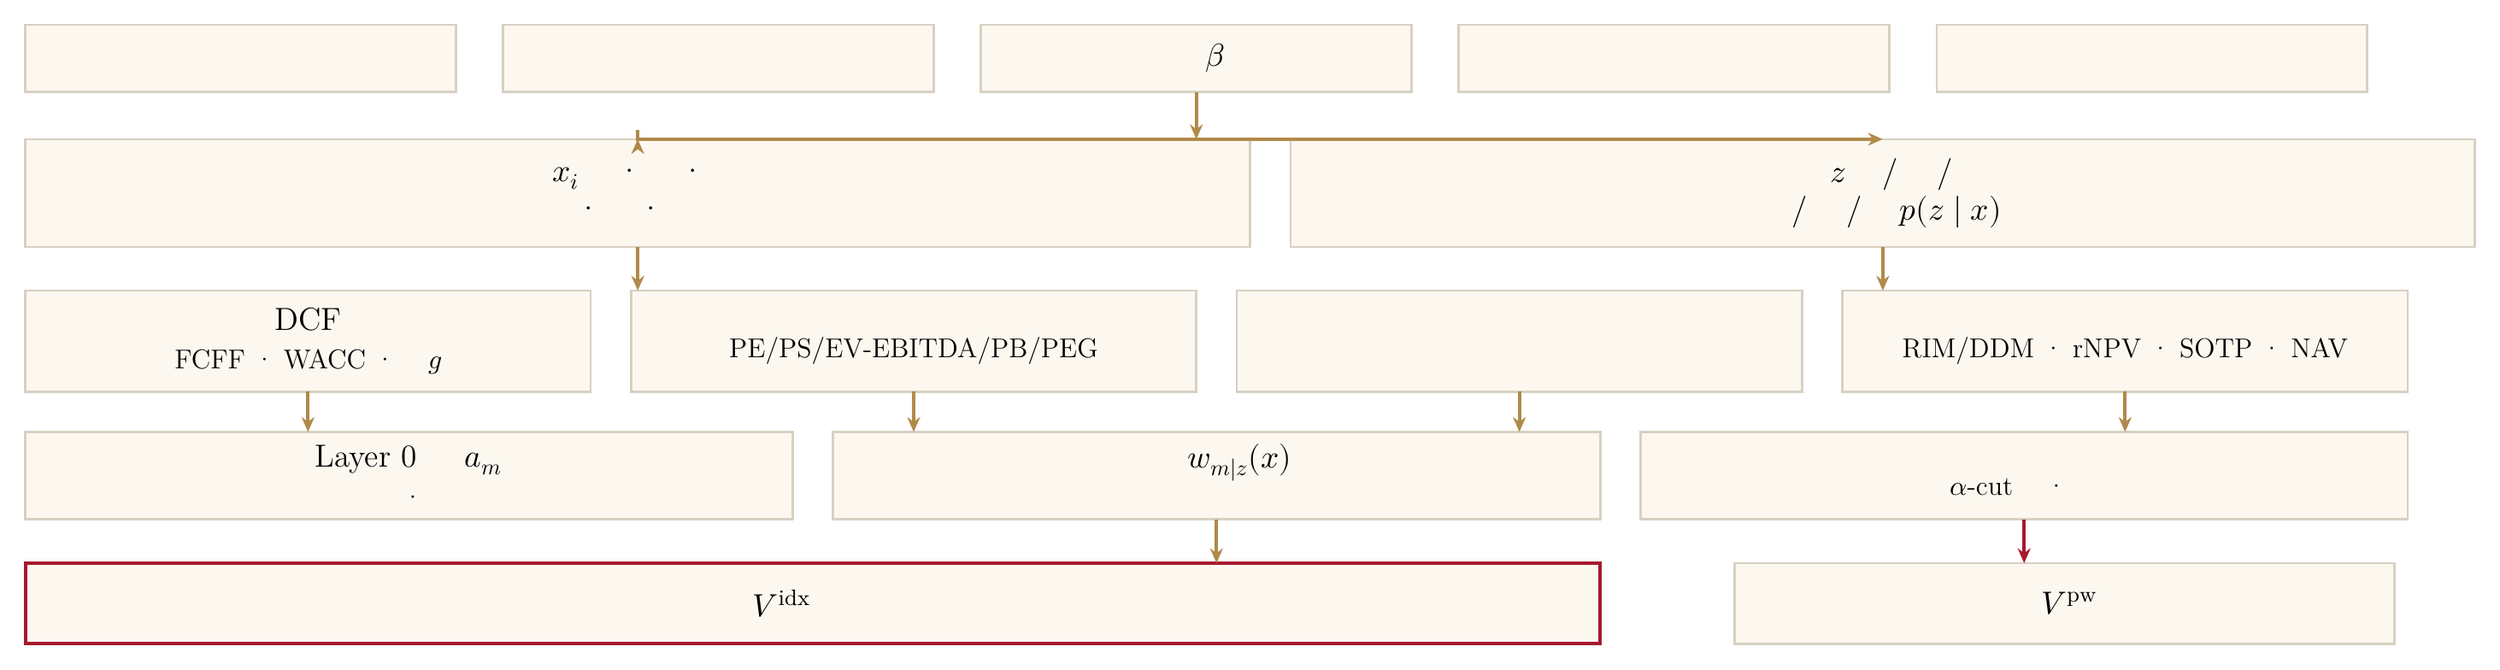
\begin{tikzpicture}[x=1mm,y=1mm,font=\song,
  bx/.style={draw=hairline,fill=creamlt,line width=0.35mm,align=center,inner sep=0.8mm,
             font=\fontsize{13.5}{16}\selectfont},
  a/.style={-{Stealth[length=2.2mm,width=1.9mm]},line width=0.5mm,gold}]
\node[bx,minimum width=64mm,minimum height=10mm] (d1) at (36,93) {成分与权重};
\node[bx,minimum width=64mm,minimum height=10mm] (d2) at (107,93) {财报与一致预期};
\node[bx,minimum width=64mm,minimum height=10mm] (d3) at (178,93) {行情与 $\beta$};
\node[bx,minimum width=64mm,minimum height=10mm] (d4) at (249,93) {舆情与股吧};
\node[bx,minimum width=64mm,minimum height=10mm] (d5) at (320,93) {行业估值基准};
\node[bx,minimum width=182mm,minimum height=16mm] (fx) at (95,73) {特征 $x_i$：行业 · 规模 · 盈利质量\\增长 · 杠杆 · 现金流稳定性};
\node[bx,minimum width=176mm,minimum height=16mm] (lz) at (280,73) {生命周期 $z$：导入 / 成长 / 成熟\\衰退 / 金融 / 周期；$p(z\mid x)$};
\draw[a] (178,88) -- (178,81);
\draw[a] (178,81) -- (95,81) -- (95,81);
\draw[a] (178,81) -- (280,81);
\node[bx,minimum width=84mm,minimum height=15mm] (m1) at (46,51) {DCF\\[0.2mm]{\fontsize{11.5}{13}\selectfont FCFF · WACC · 永续 $g$}};
\node[bx,minimum width=84mm,minimum height=15mm] (m2) at (136,51) {可比\\[0.2mm]{\fontsize{11.5}{13}\selectfont \mbox{PE/PS/EV-EBITDA/PB/PEG}}};
\node[bx,minimum width=84mm,minimum height=15mm] (m3) at (226,51) {舆情\\[0.2mm]{\fontsize{11.5}{13}\selectfont 词频 或 语义权重}};
\node[bx,minimum width=84mm,minimum height=15mm] (m4) at (316,51) {金融与特殊\\[0.2mm]{\fontsize{11.5}{13}\selectfont RIM/DDM · rNPV · SOTP · NAV}};
\draw[a] (95,65) -- (95,58.5);
\draw[a] (280,65) -- (280,58.5);
\node[bx,minimum width=114mm,minimum height=13mm] (g1) at (61,31) {Layer 0 前提门 $a_m$\\[0.2mm]{\fontsize{11.5}{13}\selectfont 数据充分性 · 适用边界}};
\node[bx,minimum width=114mm,minimum height=13mm] (g2) at (181,31) {门控权重 $w_{m\mid z}(x)$\\[0.2mm]{\fontsize{11.5}{13}\selectfont 生命周期层内归一}};
\node[bx,minimum width=114mm,minimum height=13mm] (g3) at (301,31) {模糊加权与合成\\[0.2mm]{\fontsize{11.5}{13}\selectfont $\alpha$-cut 传播 · 线性池}};
\draw[a] (46,43.5) -- (46,37.5);
\draw[a] (136,43.5) -- (136,37.5);
\draw[a] (226,43.5) -- (226,37.5);
\draw[a] (316,43.5) -- (316,37.5);
\node[bx,draw=lacquer,line width=0.5mm,minimum width=234mm,minimum height=12mm] (o1) at (121,12) {拟合点位 $V^{\mathrm{idx}}$：与收盘并列，差异只诊断};
\node[bx,minimum width=98mm,minimum height=12mm] (o2) at (307,12) {价格加权 $V^{\mathrm{pw}}$（对照）};
\draw[a,draw=lacquer] (301,24.5) -- (301,18);
\draw[a] (181,24.5) -- (181,18);
\end{tikzpicture}\par}
\vspace{-3mm}
\figcap{图 1\quad 逐券估值到点位合成的数据流：门控在生命周期层内完成，方法不可用即剔除，合成按指数权重归一。}

% ---------------- 三 ----------------
\sect{三、}{有界多智能体校准}

参数（可比权重、舆情权重、WACC 或 $K_e$、永续增速）不由模型自由生成。三名专家各审一个证据域——可比质量、折现参数、舆情——只提本域参数；主审独立复核，给出 accept / clamp / reject。门槛是硬的：置信度 $\geq 0.65$、引用具体数字、severity 与幅度匹配、方向自洽；未过门槛只留痕。

幅度上限：可比 5/8/10pp、舆情 5/10pp、WACC 0.4/1.0pp、永续 0.2/0.6pp；权重按 5pp、WACC 与永续按 0.2pp 取网格。

\eqbox{%
{\fontsize{21}{26}\selectfont
\begin{align}
T_{\mathrm{apply}}(x)&=F\bigl(x;\theta+A\,R\,G\,\Pi(e)\bigr),\qquad T_{\mathrm{shadow}}(x)=F(x;\theta),\label{eq:T}\\
\delta^\star&=\arg\min_{\delta\in\mathcal C}\ \mathcal L(\theta+\delta;e)+\lambda\|\delta\|_1,\qquad
\mathcal C=\{\delta:|\delta_j|\le c_j(s),\ \theta+\delta\in\Theta_{\mathrm{feas}}\}.\label{eq:delta}
\end{align}}
{\fontsize{15.5}{20}\selectfont\color{stone}(4)：$A$ 采纳门、$R$ 幅度约束、$G$ 网格化、$\Pi(e)$ 证据投影；$\delta$ 被限制在信赖域 $\mathcal C$ 内。}\par}

shadow 只留痕；apply 回写输入并重跑引擎，保留 baseline，失败回滚。自迭代 $\theta_{t+1}=\theta_t+\eta_tA_t\delta_t^\star$ 属论文扩展。

% 协议图
\vspace{-1mm}{\centering
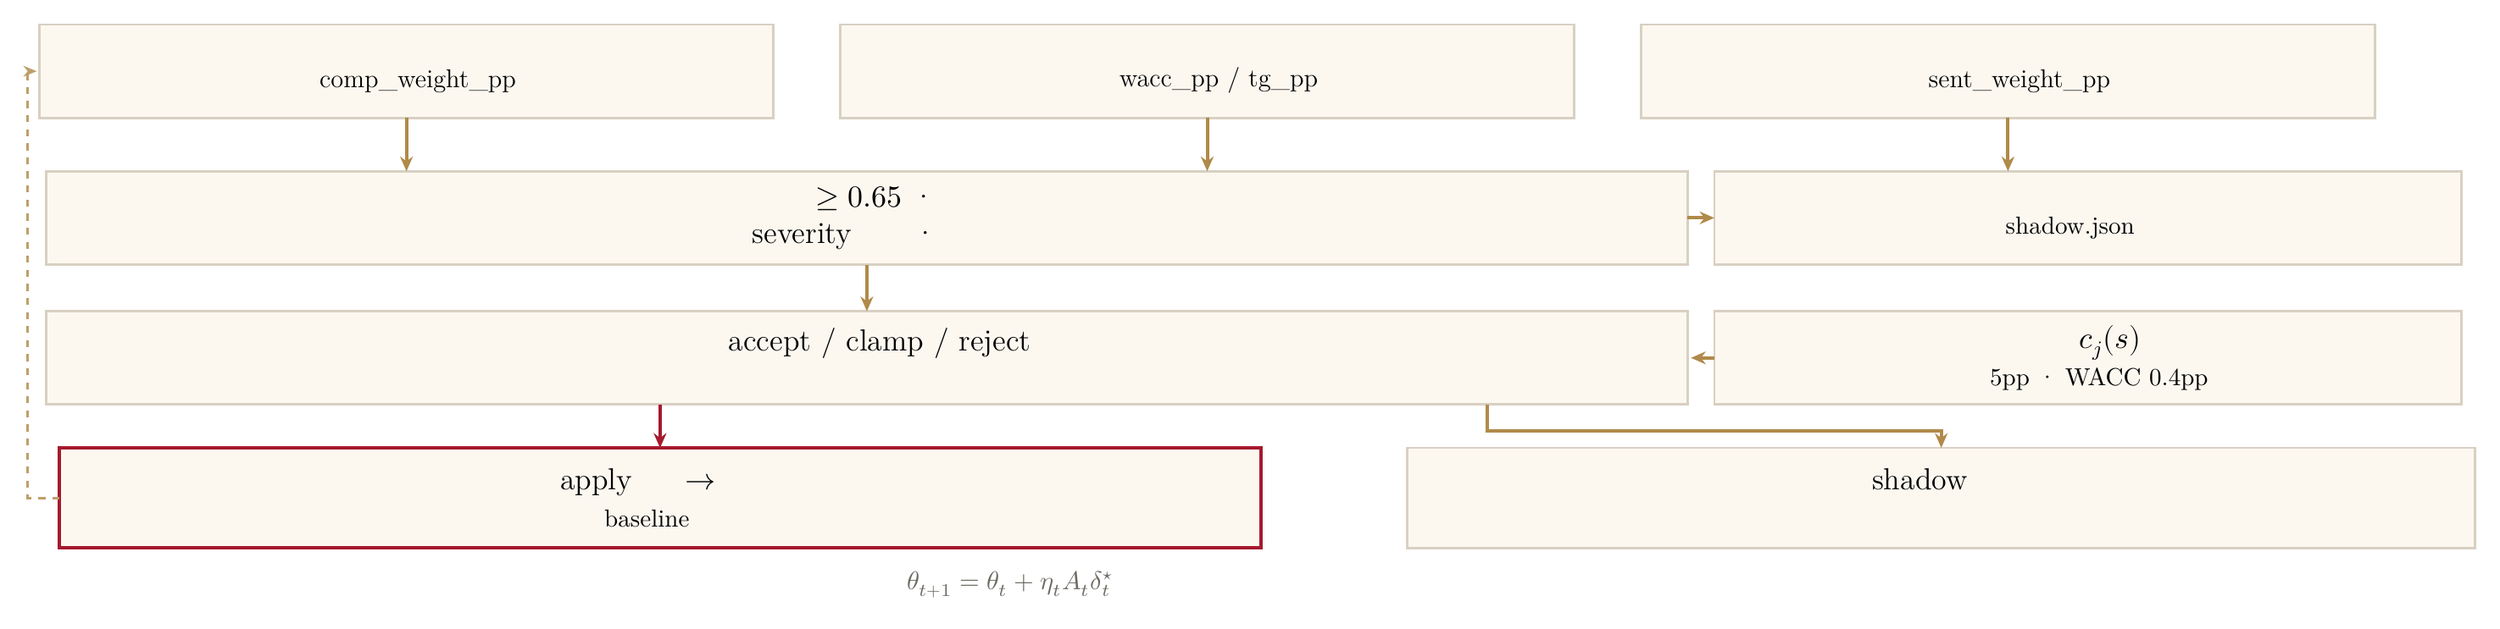
\begin{tikzpicture}[x=1mm,y=1mm,font=\song,
  bx/.style={draw=hairline,fill=creamlt,line width=0.35mm,align=center,inner sep=0.7mm,
             font=\fontsize{13}{15.5}\selectfont},
  a/.style={-{Stealth[length=2.2mm,width=1.9mm]},line width=0.5mm,gold}]
\node[bx,minimum width=110mm,minimum height=14mm] (e1) at (58,85) {可比专家\\[0.2mm]{\fontsize{11}{13}\selectfont 只提 comp\_weight\_pp}};
\node[bx,minimum width=110mm,minimum height=14mm] (e2) at (178,85) {折现专家\\[0.2mm]{\fontsize{11}{13}\selectfont 只提 wacc\_pp / tg\_pp}};
\node[bx,minimum width=110mm,minimum height=14mm] (e3) at (298,85) {舆情专家\\[0.2mm]{\fontsize{11}{13}\selectfont 只提 sent\_weight\_pp}};
\node[bx,minimum width=246mm,minimum height=14mm] (th) at (127,63) {证据门槛：置信度 $\geq 0.65$ · 引用具体数字\\severity 与幅度匹配 · 方向自洽};
\node[bx,minimum width=112mm,minimum height=14mm] (sh) at (310,63) {未过门槛：只留痕\\[0.2mm]{\fontsize{10.5}{12}\selectfont shadow.json 逐券记录}};
\node[bx,minimum width=246mm,minimum height=14mm] (ch) at (127,42) {主审：accept / clamp / reject\\[0.2mm]{\fontsize{11}{13}\selectfont 独立复核，不新增参数}};
\node[bx,minimum width=112mm,minimum height=14mm] (cap) at (310,42) {幅度上限 $c_j(s)$\\[0.2mm]{\fontsize{10.5}{12}\selectfont 权重 5pp · WACC 0.4pp}};
\node[bx,draw=lacquer,line width=0.5mm,minimum width=180mm,minimum height=15mm] (ap) at (96,21) {apply：写回输入 $\rightarrow$ 重跑引擎\\[0.2mm]{\fontsize{10.5}{12}\selectfont 保留 baseline，失败自动回滚}};
\node[bx,minimum width=160mm,minimum height=15mm] (sc) at (288,21) {shadow：不改参数\\[0.2mm]{\fontsize{10.5}{12}\selectfont 仅供比较与人工采纳}};
\draw[a] (58,78) -- (58,70);
\draw[a] (178,78) -- (178,70);
\draw[a] (298,78) -- (298,70);
\draw[a] (127,56) -- (127,49);
\draw[a] (250,63) -- (254,63);
\draw[a] (254,42) -- (250.5,42);
\draw[a,draw=lacquer] (96,35) -- (96,28.5);
\draw[a] (220,35) -- (220,31) -- (288,31) -- (288,28.5);
\node[font=\fontsize{11}{13}\selectfont,text=stone,align=center] at (150,8) {虚线为自迭代 $\theta_{t+1}=\theta_t+\eta_tA_t\delta_t^\star$（论文扩展，未上线）};
\draw[-{Stealth[length=2mm,width=1.6mm]},dashed,line width=0.4mm,gold!80!cream] (6,21) -- (1.2,21) -- (1.2,85) -- (2.6,85);
\end{tikzpicture}\par}
\vspace{-3mm}
\figcap{图 2\quad 有界评审协议：专家只动本域参数，主审在幅度上限与信赖域内裁决；apply / shadow 双轨，全程可回滚、可审计。}

\end{minipage}%
\hspace*{\gut}%
\begin{minipage}[t]{\colw}\RaggedRight
% ---------------- 四 ----------------
\sect{四、}{五指数与数据}

覆盖上证50、上证180、科创50、沪深300 与上证综指。前四者取成分表前一日收盘权重，缺权重时以自由流通市值归一并在前端标注；上证综指走全市场快照、总市值权重，剔除 ST/*ST 与未满计入期新股（上市满一年计入，总市值前 10 名满三个月）。

\vspace{0.5mm}
{\fontsize{19.5}{26}\selectfont\renewcommand{\arraystretch}{1.28}
\begin{tabular}{@{}p{58mm}r@{\hspace{6mm}}p{148mm}p{112mm}@{}}
\toprule[1.1mm]
{\thd 指数} & {\thd 样本数} & {\thd 权重口径} & {\thd 数据时点}\\
\midrule[0.45mm]
上证50 & 50 & 成分表权重 & 前一日收盘\\
\arrayrulecolor{hairline}\midrule[0.15mm]
上证180 & 180 & 成分表权重 & 前一日收盘\\
\midrule[0.15mm]
科创50 & 50 & 成分表权重 & 前一日收盘\\
\midrule[0.15mm]
沪深300 & 300 & 成分表权重（缺则自由流通市值归一） & 前一日收盘\\
\midrule[0.15mm]
上证综指 & 2{,}201 & 总市值权重，剔除 ST/*ST 与未满计入期新股 & 全市场快照\\
\bottomrule[1.1mm]
\end{tabular}}

\tabnote{表 1\quad 指数范围与权重口径。单样本 15\% 上限当前未显式截断（样本远低于上限，正式口径待核实）。}

数据来自东方财富（成分、财报、F10、行业估值）、腾讯行情、东财新闻与股吧，公开披露，无付费数据依赖；缓存按 5 分钟至 7 天分级。全市场按券起 4 个子进程（引擎、统计、报告、机检），并行 3 或 10。

权重与市值的关系尚未按“权重因子 $\times$ 当日市值”逐日重算，当前直接使用成分表权重；估值时点也尚未真正 PIT——前端日期仅作参考，批跑固定使用成分数据时点。这两步是正式口径前必须闭环的部分。

% ---------------- 五 ----------------
\sect{五、}{示例证据}

技能包随附四个参考案例，用于展示输出形态与证据链，不用以证明准确率。

\vspace{0.5mm}
{\fontsize{19.5}{26}\selectfont\renewcommand{\arraystretch}{1.28}
\begin{tabular}{@{}p{54mm}p{130mm}r@{\hspace{9mm}}p{80mm}p{28mm}@{}}
\toprule[1.1mm]
{\thd 案例} & {\thd 行业} & {\thd 中枢} & {\thd 区间} & {\thd 置信度}\\
\midrule[0.45mm]
芯曜微电 & AI 芯片设计（Fabless） & 271.23 & 149.81–423.03 & 高\\
\arrayrulecolor{hairline}\midrule[0.15mm]
长鑫科技 & 半导体 & 3{,}425.67 & 1{,}630.64–5{,}659.13 & 高\\
\midrule[0.15mm]
天博智能 & 汽车热管理零部件 & 123.62 & 53.57–216.45 & 高\\
\midrule[0.15mm]
宇树科技 & 人形 / 四足机器人 & 972.42 & 569.24–1{,}446.64 & 高\\
\bottomrule[1.1mm]
\end{tabular}}

\tabnote{表 2\quad 参考案例的中枢与区间（单位：亿元）。技能包示例案例，不是指数级回测；置信度为引擎输出，样本为示例、非随机抽样。四例覆盖 AI 芯片设计、存储制造、汽车零部件与人形机器人；区间为引擎输出，不含对未来的预测。}

\lead{系统证据}
{\fontsize{21}{28}\selectfont
\begin{itemize}\setlength{\itemsep}{0.8mm}\setlength{\parsep}{0pt}\setlength{\topsep}{1mm}\setlength{\leftmargin}{5mm}
\item 回归：\texttt{smoke\_test.py} 实跑 170 用例全绿（约 4 秒），引擎版本 2.28.0。
\item 报告：11 段投行级 HTML、8 项机检；每券 4 个子进程（引擎 / 统计 / 报告 / 机检）。
\item 交付：10 个脚本、27 个示例文件（11 input / 9 output / 7 stat）。
\item 每券留痕：\texttt{shadow.json}、\texttt{summary.html}、11 段报告与 8 项机检。
\end{itemize}}

\lead{评估协议（无真值）}
{\fontsize{21}{28}\selectfont
\begin{itemize}\setlength{\itemsep}{0.8mm}\setlength{\parsep}{0pt}\setlength{\topsep}{1mm}\setlength{\leftmargin}{5mm}
\item \textbf{合成基准}：注入已知 $V_i^\star$，再注入财报错误、可比缺失与路由错误，测恢复误差、区间覆盖与路由准确。
\item \textbf{人工盲评}：隐藏建议与点位，4–6 人独立评证据、方向、幅度与置信；两轮 Delphi 后仲裁，报 Krippendorff $\alpha$。
\item \textbf{内部一致性}：同输入多 seed、股票排列、单位缩放、行业标签扰动；shadow 空操作、apply 回滚、8 项机检。
\end{itemize}}

% ---------------- 六 ----------------
\sect{六、}{讨论与启示}

\lead{对指数编制}　估值读数可作为“基本面锚”的旁证指标，用于极端偏离筛查与编制方案的压力测试；它不替代收盘点位，也不进入指数计算。

\lead{对估值研究}　无真值条件下，评估重心应从“拟合收盘”转向一致性、区间校准与可复现；市场指标只作诊断，不能既当裁判又当运动员。

\lead{对监管披露}　参数改动留痕、baseline 可回滚、逐券 shadow 记录，使“模型改了什么”成为可审计对象，而不只是结果数字。

\lead{局限}
{\fontsize{21}{28}\selectfont
\begin{itemize}\setlength{\itemsep}{0.8mm}\setlength{\parsep}{0pt}\setlength{\topsep}{1mm}\setlength{\leftmargin}{5mm}
\item 无真值：没有可用的监督信号，只能靠一致性、区间校准与盲评三角验证。
\item 时点与数据：估值时点未真正 PIT；公开接口无 SLA，字段与限频可能变。
\item 随机性：LLM 评审 temperature 0.1 但无 seed，建议分布的方差未量化。
\item 循环论证：专家证据与引擎输入同源，需外部证据与盲评补强。
\end{itemize}}

\lead{下一步}　PIT 数据层；三池（训练 / 验证 / 影子）；技能拆分与向量化取数；编制口径正式化（单样本 15\% 上限）。

% ---------------- 七 ----------------
\sect{七、}{结论}

{\fontsize{23}{30}\selectfont
\begin{enumerate}\setlength{\itemsep}{1.2mm}\setlength{\topsep}{1mm}\setlength{\leftmargin}{6mm}
\item 估值合成是价格合成之外的一种可计算口径：同一组权重、不同的“原子”，差异可分解、可诊断。
\item 参数校准必须有界：证据门槛、幅度上限、信赖域、shadow/apply 与回滚，把“模型改了什么”变成审计对象。
\item 系统已覆盖五指数、2,201 只、170 项回归；下一步是补齐 PIT、盲评与参数学习，而不是追求贴近收盘。
\end{enumerate}}

\end{minipage}

% =====================================================================
% 页脚
% =====================================================================
\par\vfill
\noindent\hspace*{\bodymargin}%
\parbox[b]{800mm}{%
{\color{gold}\rule{800mm}{0.45mm}}\par\vspace{3mm}
\parbox[t]{716mm}{\vspace{0pt}\raggedright
{\fontsize{16}{22}\selectfont\color{stone}本文为探索性研究，观点属作者个人，不代表中证指数有限公司立场。示例案例不是指数级回测，样本非随机，不构成投资建议。数据来自东方财富、腾讯行情及公开披露。通信作者：宋泊毅，bysong@sse.com.cn}}\hfill
\parbox[t]{58mm}{\vspace{0pt}\centering

\begin{tikzpicture}[x=0.8mm,y=0.8mm]
\fill[white] (-1.6,-1.6) rectangle (30.6,30.6);
\begin{scope}
\color{ink}
\fill (0,28) rectangle (7,29);
\fill (9,28) rectangle (10,29);
\fill (12,28) rectangle (13,29);
\fill (15,28) rectangle (16,29);
\fill (18,28) rectangle (20,29);
\fill (22,28) rectangle (29,29);
\fill (0,27) rectangle (1,28);
\fill (6,27) rectangle (7,28);
\fill (10,27) rectangle (16,28);
\fill (17,27) rectangle (21,28);
\fill (22,27) rectangle (23,28);
\fill (28,27) rectangle (29,28);
\fill (0,26) rectangle (1,27);
\fill (2,26) rectangle (5,27);
\fill (6,26) rectangle (7,27);
\fill (8,26) rectangle (11,27);
\fill (12,26) rectangle (13,27);
\fill (20,26) rectangle (21,27);
\fill (22,26) rectangle (23,27);
\fill (24,26) rectangle (27,27);
\fill (28,26) rectangle (29,27);
\fill (0,25) rectangle (1,26);
\fill (2,25) rectangle (5,26);
\fill (6,25) rectangle (7,26);
\fill (9,25) rectangle (12,26);
\fill (14,25) rectangle (15,26);
\fill (18,25) rectangle (19,26);
\fill (20,25) rectangle (21,26);
\fill (22,25) rectangle (23,26);
\fill (24,25) rectangle (27,26);
\fill (28,25) rectangle (29,26);
\fill (0,24) rectangle (1,25);
\fill (2,24) rectangle (5,25);
\fill (6,24) rectangle (7,25);
\fill (10,24) rectangle (11,25);
\fill (14,24) rectangle (16,25);
\fill (18,24) rectangle (20,25);
\fill (22,24) rectangle (23,25);
\fill (24,24) rectangle (27,25);
\fill (28,24) rectangle (29,25);
\fill (0,23) rectangle (1,24);
\fill (6,23) rectangle (7,24);
\fill (9,23) rectangle (10,24);
\fill (13,23) rectangle (14,24);
\fill (15,23) rectangle (21,24);
\fill (22,23) rectangle (23,24);
\fill (28,23) rectangle (29,24);
\fill (0,22) rectangle (7,23);
\fill (8,22) rectangle (9,23);
\fill (10,22) rectangle (11,23);
\fill (12,22) rectangle (13,23);
\fill (14,22) rectangle (15,23);
\fill (16,22) rectangle (17,23);
\fill (18,22) rectangle (19,23);
\fill (20,22) rectangle (21,23);
\fill (22,22) rectangle (29,23);
\fill (8,21) rectangle (11,22);
\fill (12,21) rectangle (16,22);
\fill (17,21) rectangle (19,22);
\fill (20,21) rectangle (21,22);
\fill (0,20) rectangle (3,21);
\fill (4,20) rectangle (9,21);
\fill (10,20) rectangle (14,21);
\fill (16,20) rectangle (23,21);
\fill (26,20) rectangle (27,21);
\fill (1,19) rectangle (3,20);
\fill (4,19) rectangle (5,20);
\fill (10,19) rectangle (12,20);
\fill (13,19) rectangle (15,20);
\fill (16,19) rectangle (19,20);
\fill (20,19) rectangle (21,20);
\fill (22,19) rectangle (23,20);
\fill (25,19) rectangle (26,20);
\fill (28,19) rectangle (29,20);
\fill (1,18) rectangle (2,19);
\fill (4,18) rectangle (8,19);
\fill (9,18) rectangle (10,19);
\fill (12,18) rectangle (13,19);
\fill (16,18) rectangle (19,19);
\fill (20,18) rectangle (23,19);
\fill (24,18) rectangle (25,19);
\fill (26,18) rectangle (29,19);
\fill (0,17) rectangle (1,18);
\fill (3,17) rectangle (4,18);
\fill (11,17) rectangle (12,18);
\fill (13,17) rectangle (14,18);
\fill (16,17) rectangle (18,18);
\fill (23,17) rectangle (25,18);
\fill (27,17) rectangle (28,18);
\fill (0,16) rectangle (7,17);
\fill (8,16) rectangle (9,17);
\fill (11,16) rectangle (12,17);
\fill (13,16) rectangle (14,17);
\fill (17,16) rectangle (19,17);
\fill (20,16) rectangle (23,17);
\fill (25,16) rectangle (26,17);
\fill (27,16) rectangle (29,17);
\fill (0,15) rectangle (2,16);
\fill (3,15) rectangle (6,16);
\fill (8,15) rectangle (9,16);
\fill (12,15) rectangle (13,16);
\fill (16,15) rectangle (23,16);
\fill (25,15) rectangle (26,16);
\fill (28,15) rectangle (29,16);
\fill (2,14) rectangle (3,15);
\fill (5,14) rectangle (8,15);
\fill (9,14) rectangle (10,15);
\fill (14,14) rectangle (15,15);
\fill (18,14) rectangle (19,15);
\fill (22,14) rectangle (23,15);
\fill (24,14) rectangle (26,15);
\fill (27,14) rectangle (29,15);
\fill (0,13) rectangle (1,14);
\fill (4,13) rectangle (5,14);
\fill (9,13) rectangle (10,14);
\fill (11,13) rectangle (18,14);
\fill (20,13) rectangle (23,14);
\fill (25,13) rectangle (26,14);
\fill (27,13) rectangle (28,14);
\fill (0,12) rectangle (1,13);
\fill (4,12) rectangle (8,13);
\fill (9,12) rectangle (10,13);
\fill (12,12) rectangle (14,13);
\fill (15,12) rectangle (21,13);
\fill (22,12) rectangle (24,13);
\fill (25,12) rectangle (26,13);
\fill (27,12) rectangle (29,13);
\fill (3,11) rectangle (4,12);
\fill (5,11) rectangle (6,12);
\fill (12,11) rectangle (13,12);
\fill (17,11) rectangle (19,12);
\fill (21,11) rectangle (23,12);
\fill (25,11) rectangle (27,12);
\fill (28,11) rectangle (29,12);
\fill (0,10) rectangle (1,11);
\fill (6,10) rectangle (7,11);
\fill (12,10) rectangle (14,11);
\fill (17,10) rectangle (19,11);
\fill (21,10) rectangle (22,11);
\fill (23,10) rectangle (25,11);
\fill (27,10) rectangle (29,11);
\fill (1,9) rectangle (2,10);
\fill (4,9) rectangle (5,10);
\fill (9,9) rectangle (10,10);
\fill (11,9) rectangle (15,10);
\fill (16,9) rectangle (18,10);
\fill (19,9) rectangle (26,10);
\fill (27,9) rectangle (28,10);
\fill (0,8) rectangle (1,9);
\fill (6,8) rectangle (7,9);
\fill (9,8) rectangle (10,9);
\fill (12,8) rectangle (14,9);
\fill (15,8) rectangle (25,9);
\fill (8,7) rectangle (9,8);
\fill (12,7) rectangle (13,8);
\fill (16,7) rectangle (21,8);
\fill (24,7) rectangle (25,8);
\fill (26,7) rectangle (29,8);
\fill (0,6) rectangle (7,7);
\fill (8,6) rectangle (9,7);
\fill (10,6) rectangle (11,7);
\fill (12,6) rectangle (14,7);
\fill (16,6) rectangle (21,7);
\fill (22,6) rectangle (23,7);
\fill (24,6) rectangle (26,7);
\fill (27,6) rectangle (29,7);
\fill (0,5) rectangle (1,6);
\fill (6,5) rectangle (7,6);
\fill (8,5) rectangle (9,6);
\fill (10,5) rectangle (11,6);
\fill (12,5) rectangle (14,6);
\fill (15,5) rectangle (16,6);
\fill (17,5) rectangle (18,6);
\fill (20,5) rectangle (21,6);
\fill (24,5) rectangle (26,6);
\fill (27,5) rectangle (28,6);
\fill (0,4) rectangle (1,5);
\fill (2,4) rectangle (5,5);
\fill (6,4) rectangle (7,5);
\fill (8,4) rectangle (15,5);
\fill (17,4) rectangle (19,5);
\fill (20,4) rectangle (25,5);
\fill (28,4) rectangle (29,5);
\fill (0,3) rectangle (1,4);
\fill (2,3) rectangle (5,4);
\fill (6,3) rectangle (7,4);
\fill (12,3) rectangle (13,4);
\fill (16,3) rectangle (17,4);
\fill (20,3) rectangle (21,4);
\fill (23,3) rectangle (25,4);
\fill (26,3) rectangle (27,4);
\fill (28,3) rectangle (29,4);
\fill (0,2) rectangle (1,3);
\fill (2,2) rectangle (5,3);
\fill (6,2) rectangle (7,3);
\fill (8,2) rectangle (11,3);
\fill (17,2) rectangle (18,3);
\fill (19,2) rectangle (20,3);
\fill (23,2) rectangle (26,3);
\fill (28,2) rectangle (29,3);
\fill (0,1) rectangle (1,2);
\fill (6,1) rectangle (7,2);
\fill (8,1) rectangle (10,2);
\fill (11,1) rectangle (12,2);
\fill (13,1) rectangle (16,2);
\fill (17,1) rectangle (22,2);
\fill (24,1) rectangle (25,2);
\fill (27,1) rectangle (28,2);
\fill (0,0) rectangle (7,1);
\fill (8,0) rectangle (14,1);
\fill (15,0) rectangle (18,1);
\fill (19,0) rectangle (22,1);
\fill (23,0) rectangle (25,1);
\fill (27,0) rectangle (29,1);
\end{scope}
\end{tikzpicture}\par\vspace{1.4mm}
{\fontsize{10.5}{12}\selectfont\color{stone}仓库 · 复现}}}
\vspace*{5mm}

\end{document}